\documentclass[a4paper,10pt]{article}

\usepackage{graphicx}
\graphicspath{ {images/} }
\usepackage[ansinew]{inputenc}
\usepackage[spanish]{babel}
\usepackage{listings}
\usepackage{color}
\usepackage{framed}
\usepackage{graphicx}
\usepackage{mathtools}
\usepackage{amsmath}
\usepackage{epstopdf}
\usepackage[T1]{fontenc}

\definecolor{dkgreen}{rgb}{0,0.6,0}
\definecolor{gray}{rgb}{0.5,0.5,0.5}
\definecolor{mauve}{rgb}{0.58,0,0.82}

\lstset{ %
  language=C,                       % the language of the code
  basicstyle=\footnotesize,         % the size of the fonts that are used for the code
  numbers=left,                     % where to put the line-numbers
  numberstyle=\tiny\color{gray},    % the style that is used for the line-numbers
  stepnumber=1,                     % the step between two line-numbers. If it's 1, each line 
                                    % will be numbered
  numbersep=5pt,                    % how far the line-numbers are from the code
  backgroundcolor=\color{white},    % choose the background color. You must add \usepackage{color}
  showspaces=false,                 % show spaces adding particular underscores
  showstringspaces=false,           % underline spaces within strings
  showtabs=false,                   % show tabs within strings adding particular underscores
  frame=single,                     % adds a frame around the code
  rulecolor=\color{black},          % if not set, the frame-color may be changed on line-breaks within not-black text (e.g. commens (green here))
  tabsize=2,                        % sets default tabsize to 2 spaces
  captionpos=b,                     % sets the caption-position to bottom
  breaklines=true,                  % sets automatic line breaking
  breakatwhitespace=false,          % sets if automatic breaks should only happen at whitespace
  title=\lstname,                   % show the filename of files included with \lstinputlisting;
                                    % also try caption instead of title
  keywordstyle=\color{blue},        % keyword style
  commentstyle=\color{dkgreen},     % comment style
  stringstyle=\color{mauve},        % string literal style
  escapeinside={\%*}{*)},           % if you want to add LaTeX within your code
  morekeywords={*,...},             % if you want to add more keywords to the set
  rulesepcolor=\color{blue}
}

\title{     \textbf{Trabajo Práctico 1: \\ Conjunto de instrucciones MIPS}}

\author{
            Jimenez, Ruben, \textit{Padrón Nro. 92.402}                            \\
            \texttt{ rbnm.jimenez@gmail.com }                                   \\[2.5ex]
            Reyero, Felix, \textit{Padrón Nro. 92.979}                             \\
            \texttt{ felixcarp@gmail.com }                                    \\[2.5ex]
            Suárez, Emiliano, \textit{Padrón Nro. 78.372}                             \\
            \texttt{ emilianosuarez@gmail.com }                                    \\[2.5ex]
    Primera Entrega: \textit{30/04/2015}                                            \\[1.5ex]
            \normalsize{1er. Cuatrimestre de 2015}                                  \\
            \normalsize{66.20 Organización de Computadoras  $-$ Práctica Jueves}    \\
            \normalsize{Facultad de Ingeniería, Universidad de Buenos Aires}        \\
       }
\date{}

\begin{document}

\maketitle
\thispagestyle{empty}   % quita el número en la primer página

\newpage
\begin{abstract}
Se implementó una versión simplificada del programa \textbf{sha1} de UNIX. Para nuestra implementación.
\end{abstract}

\section{Introducción}

Este Trabajo Práctico pretende familiarizarse con la programación en assembly y el concepto de ABI.

Para ello, implementaremos el algoritmo \textbf{sha1} de UNIX en código \textsl{Assembly}, mientras que la interpretación de argumentos del programa y la lectura de archivos será realizada en lenguaje \textsl{C}.

Además, se utilizará \textsl{GXemul} para simular una máquina \textsl{MIPS} corriendo una versión reciente del sistema operativo \textsl{NetBSD}.

El programa implementado, muestra por \textsl{stdout} un checksum generado a partir del contenido de los archivos archivos pasados por parámetro. En caso de no especificarse algún archivo, se mostrarán un checksum a partir de lo ingresado por \textsl{stdin}.

\newpage
\section{Diseño e Implementación}

Se implementó un programa que realiza la lectura a través del stdin o a través de archivos que se reciben por parámetro.

El comando acepta 2 parámetros para mostrar la Ayuda y la Versión del programa:
\begin{verbatim}
$ ./tp1 -h
$ ./tp1 --help
\end{verbatim}
Para desplegar la ayuda del comando.
Y los siguientes comandos para mostrar la versión:
\begin{verbatim}
$ ./tp1 -V
$ ./tp1 --version
\end{verbatim}

Inicialmente el programa revisa la cadena de parametros ingresada y determina si el checksum debe generarse a partir de lo ingresado por \textsl{stdin} o a través del contenido del (o los) archivo(s).

Para este última opción, se procesan los archivo de uno por vez, y para cada uno de ellos se genera el checksum a partir de sus datos.

Las funciones \textsl{sha1} y \textsl{cargarTrozos} (llamada desde la primer función mencionada), fueron implementadas en leguanje \textsl{Assembly}. Cada una de ellas con su corresponientes stack que puede observase a continuación:

\begin{center}
    \begin{tabular}{ | p{3cm} | p{3cm}  | }
    \hline
        Dir Mem & Valor \\ \hline
        100 &  \\ \hline
        96 & ra \\ \hline
        92 & fp \\ \hline
        88 & gp \\ \hline
        84 &  \\ \hline
        80 & mascara \\ \hline
        76 & temp \\ \hline
        72 & k \\ \hline
        68 & fp \\ \hline
        64 & i \\ \hline
        60 & indice \\ \hline
        56 & E \\ \hline
        52 & D \\ \hline
        48 & C \\ \hline
        44 & B \\ \hline
        40 & A \\ \hline
        36 & cantBloques \\ \hline
        32 & cantBloques \\ \hline
        28 & longOrig \\ \hline
        24 & longOrig \\ \hline
        20 & longRelleno \\ \hline
        16 & longRelleno \\ \hline
        12 & a3 \\ \hline
        8 & a2 \\ \hline
        4 & a1 \\ \hline
        0 & a0 \\ \hline
        \hline
    \end{tabular}
\end{center}

\begin{center}
    \begin{tabular}{ | p{3cm} | p{3cm}  | }
    \hline
        Dir Mem & Valor \\ \hline
        s0 & bloques \\ \hline
        s1 & trozos \\ \hline
        s2 & a \\ \hline
        s3 & b \\ \hline
        s4 & c \\ \hline
        s5 & d \\ \hline
        s6 & e \\ \hline
        s7 & f \\ \hline
    \end{tabular}
\end{center}

COMPLETAR CON ALGO MAS SOBRE LA ARQUITECTURA.

Para compilar el programa se debe abrir una terminal en la carpeta donde están alojados los archivos fuentes (\textsl{src/}) y se ejecuta el siguiente comando:
\begin{verbatim}
../src$ make
\end{verbatim}
Para generar el ejecutable \textsl{tp1}.\\
\\
\textbf{make}: se encargara de compilar los archivos generando el ejecutable.

El \textsl{Makefile} puede observarse a continuación:\\
\lstinputlisting{../src/Makefile}

La compilación del programa en NetBSD (asegurando la portabilidad), puede observarse en la figura~\ref{fig006} del Apéndice.

\newpage
\section{Casos de Prueba}
Se realizaron distintas pruebas:

COMPLETAR CON ALGUNAS PRUEBAS.

\newpage
\section{Conclusiones}

El presente trabajo permitió la familiarización con las herramientas de compilación de código C y código assembly en un entorno que emula la arquitectura MIPS 32, asegurando la portabilidad del programa.

\newpage
\section{Apéndice}
\subsection{Compilación en NetBSD}

% Inclusión de una imagen
\begin{figure}[!htp]
\begin{center}
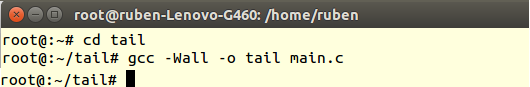
\includegraphics[width=0.7\textwidth]{test_00_compilacionGxemul}
\end{center}
\caption{Compilación NetBSD} \label{fig006}
\end{figure}

\subsection{Código Fuente: tp1.c}
\lstinputlisting{../src/tp1.c}

\end{document}
